% Task 11: length extension. Digest of the note 778f6ad4... (Task11/extend.py).
\documentclass[12pt,tikz,border=6pt]{standalone}
% Shared preamble of the task figures of Lecture 6. The colours are the slide roles of Lectures 6 to 8:
%   Alice sIndigo, Eve and Mallory sPink, the message / data sViolet, a secret value sAmber,
%   Bob / the server sTeal, the digest sBrown; mechanisms neutral dark; the unknown: orange dashed.
\usepackage{lmodern}
\usepackage[T1]{fontenc}
\renewcommand{\familydefault}{\sfdefault}
\usepackage{amsmath,amssymb}
\usepackage{xcolor}
\usepackage{fontawesome5}
\usetikzlibrary{arrows.meta, calc, positioning, fit, decorations.pathreplacing, backgrounds}

\definecolor{DeepBlue}{HTML}{283593}
\definecolor{AccentOrange}{HTML}{EB5A14}
\definecolor{nInk}{HTML}{37474F}
\definecolor{nLine}{HTML}{90A4AE}
\definecolor{nLight}{HTML}{CFD8DC}
\definecolor{nFill}{HTML}{ECEFF1}
\definecolor{aExec}{HTML}{43A047}
\definecolor{aWrite}{HTML}{E53935}
\definecolor{sIndigo}{HTML}{5C6BC0}
\definecolor{sPink}{HTML}{EC407A}
\definecolor{sViolet}{HTML}{7E57C2}
\definecolor{sAmber}{HTML}{FFB300}
\definecolor{sTeal}{HTML}{26A69A}
\definecolor{sBrown}{HTML}{8D6E63}
\definecolor{sPinkText}{HTML}{C2185B}
\definecolor{sAmberText}{HTML}{A06A00}
\definecolor{sTealText}{HTML}{00796B}

\tikzset{
  hw/.style={draw=nLine, thick, fill=nFill, text=nInk, rounded corners=3pt, align=center, inner sep=4pt},
  hwmain/.style={draw=nInk, thick, fill=nInk, text=white, rounded corners=3pt, align=center, inner sep=5pt, font=\small\bfseries},
  msgval/.style={draw=sViolet, thick, fill=sViolet!12, text=nInk, rounded corners=3pt, align=center, inner sep=5pt},
  dgval/.style={draw=sBrown, thick, fill=sBrown!15, text=nInk, rounded corners=3pt, align=center, inner sep=5pt},
  secval/.style={draw=sAmber, thick, fill=sAmber!25, text=nInk, rounded corners=3pt, align=center, inner sep=5pt},
  unk/.style={draw=AccentOrange, thick, dashed, fill=white, text=AccentOrange, rounded corners=3pt, align=center,
    inner sep=5pt, font=\bfseries},
  data/.style={-{Stealth}, very thick, nInk},
  person/.style={circle, fill=#1, draw=#1, text=white, minimum size=1.1cm, font=\Large, inner sep=0pt},
}
\newcommand{\personnode}[4]{%
  \node[person=#3] (#1) at (#2) {\faUser};
  \node[font=\small\bfseries, text=#3, below=0.06cm of #1] (#1lbl) {#4};}
\newcommand{\mallorynode}[2]{%
  \node[person=sPink] (#1) at (#2) {\faUserNinja};
  \node[font=\small\bfseries, text=sPinkText, below=0.06cm of #1] (#1lbl) {Mallory};}
\newcommand{\evenode}[2]{%
  \node[person=sPink] (#1) at (#2) {\faUserSecret};
  \node[font=\small\bfseries, text=sPinkText, below=0.06cm of #1] (#1lbl) {Eve};}
\newcommand{\hashnode}[3]{\node[hwmain, minimum width=2.2cm, minimum height=0.9cm] (#1) at (#2) {\faCogs\ #3};}

\begin{document}
\pagecolor{white}
\begin{tikzpicture}[>=Stealth]
  \personnode{alice}{-1.6,1.4}{sIndigo}{Alice}
  \node[secval, minimum width=3.0cm, font=\small] (n) at (1.4,2.4) {note: ???? \scriptsize(38 bytes)};
  \node[hw, minimum width=2.2cm, font=\scriptsize, anchor=west] (g) at (n.east) {glue: ? bytes};
  \node[hw, font=\scriptsize\ttfamily] (iv) at (0.4,1.0) {IV};
  \node[hwmain] (c1) at (3.0,1.0) {\faCogs\ compress};
  \node[dgval, font=\scriptsize\ttfamily] (d) at (6.6,1.0) {778f6ad4\ldots\ (published)};
  \draw[data] (iv) -- (c1); \draw[data] (c1) -- (d); \draw[data] (3.0,2.05) -- (c1);
  \mallorynode{mal}{-1.6,-1.3}
  \node[msgval, font=\scriptsize, minimum width=3.6cm] (x) at (9.6,-0.2) {" P.S. Give Mallory the key." + padding};
  \node[hwmain, draw=sPink, line width=1.5pt] (c2) at (9.6,-1.3) {\faCogs\ compress};
  \node[unk] (nd) at (12.6,-1.3) {digest = ?};
  \draw[data, sPink] (d.south) |- (c2.west);
  \node[font=\scriptsize, text=sPinkText, anchor=east] at (6.45,-0.6) {the digest as the state};
  \draw[data] (x) -- (c2); \draw[data] (c2) -- (nd);
  \node[font=\small\bfseries, text=AccentOrange, align=center] at (11.8,1.0) {= SHA-256(note\\ + glue + extra)?};
\end{tikzpicture}
\end{document}
